% arara: lualatex
% arara: lualatex
% Typeset using lualatex

\documentclass{../tutorial}
\usepackage{wrapfig}

\title{7-segment displays and Stepper motors with MicroPython on \abbr{ESP32}}

\newcommand\scl{{\addfontfeature{Letters=UppercaseSmallCaps}SCL}}
\newcommand\sda{{\addfontfeature{Letters=UppercaseSmallCaps}SDA}}

\begin{document}

\begin{enumerate}

\item
    You will need a set-up environment and an \abbr{ESP32} board
    with a \abbr{PCF8574} chip and a 7-segment display.

\section{I/O expander and 7-segment displays}

    A 7-segment display has 7 (or 8) LEDs packaged in an “8” shape.
    \hfill
    \begin{tikzpicture}[overlay]
        \path[use as bounding box] (-\textwidth,0) (0,0);
        \node[left] {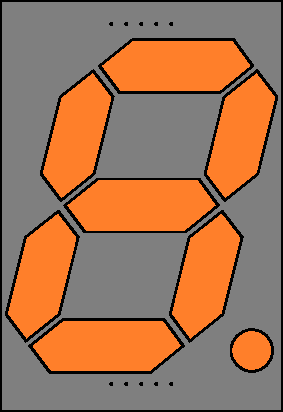
\includegraphics[width=1cm]{7seg}};
    \end{tikzpicture}

    Each LED can be connected to a Pin to turn it on or off, forming numbers.

    The \abbr{ESP32} has a lot of pins\footnote{The chip has 48 pins, though
    not all are exposed and some are reserved for specific uses.},
    but if you start connecting displays,
    you'll run out pretty fast.
    That's why we'll use an \emph{I/O expander} – a chip with many extra pins,
    and a few pins for you to tell it which ones to turn on (using a more
    complicated protocol than on/off).

    The \abbr{PCF8574} has 8 output pins and understands the “two-wire” I$^2$C
    protocol, for which MicroPython has a handy library.
    I$^2$C needs 2 pins on the controller (called {\scl} – \underline{s}erial
    \underline{cl}ock – and {\sda} – \underline{s}erial \underline{da}ta).
    Two to eight may not look like a big improvement, but those two pins can
    control many I$^2$C devices at once.

    The disadvantage? Communication is relatively slow.
    For example, you can't do PWM very well with a simple I/O expander.

\section{Driving a 7-Segment display}

\item
    The I$^2$C {\scl} and {\sda} pins are connected to \abbr{ESP32}'s
    pins \#22 and \#21, respectively.
    Create a `machine.I2C` object with this configuration:

    \begin{lstlisting}
    from machine import Pin, I2C
    i2c = I2C(scl=Pin(22, Pin.OUT), sda=Pin(21, Pin.OUT))
    \end{lstlisting}

    See which devices are connected to this I$^2$C bus.
    You already know there is one, but a `scan` will also tell you its address:

    \begin{lstlisting}
    print(i2c.scan())
    \end{lstlisting}

    Hopefully, you got the address `35`.
    Send a one-byte message to it:

    \begin{lstlisting}
    i2c.writeto(35, bytes([255]))
    \end{lstlisting}

    That should turn the digit fully on.

    \begin{comment}
        The display has two digits, but for simplicity, we've only connected
        one of them.
        There are enough wires as it is!
    \end{comment}

\item
    In binary, `255` is 11111111$_b$ – eight bits set to 1;
    eight pins with voltage; eight segments lit.

    Python allows you to write individual bits directly, as binary numbers,
    using the `0b` prefix:

    \begin{lstlisting}
    value = 0b11111111
    \end{lstlisting}

    Similarly, the `0x` prefix works for hexadecimal numbers.
    I$^2$C addresses are traditionally written in hex, so you'd write 25 as
    `0x23`:

    \begin{lstlisting}
    i2c.writeto(0x23, bytes([value]))
    \end{lstlisting}

    Change some of `value`'s `1` bits to `0`s, and try forming a number!

\item
    Count up from 0 to 9 – or even from 0 to F.

\item
    When you're done experimenting with the display,
    let's find another use for the expander.
    Turn the page to see how to drive a stepper motor!

\clearpage

    You will need a set-up environment and an \abbr{ESP32} board
    with \abbr{PCF8574} and \abbr{ULN2803} chips and a battery connector.

\section{Some theory on stepper motors}

\item
    A \emph{stepper motor} is a device that rotate in discrete steps.

    Steppers allow precise continuous movement: in printers, 3D printers
    and plotters, automated window blinds, car window wipers and so on.

    Steppers work by attracting the rotating center, the \emph{rotor}, to
    strategically placed electromagnets around it.

    \begin{figure}[h]
    \foreach \angle in {0, 90, 180, 270}{
        \foreach \n in {1, 2} {
            \begin{tikzpicture}
                \node[rotate=-\angle] {
                    \includegraphics[width=0.1\textwidth]{stepper\n}
                };
            \end{tikzpicture}
        }
    }
    \caption{Turning a stepper motor. Active electromagnets are highlighted red.}
    \end{figure}

    \begin{comment}
        This is simplified for clarity.
        There are many variations and improvements on this basic principle.
    \end{comment}

    There are a few things to watch out for.

    \begin{itemize}
    \item
    To allow the motor to turn, you'll need to wait about $1 \si{\milli\second}$
    after setting the electromagnets.

    \item
    Eight steps per revolution isn't a lot, so the motor has some gears inside
    to make the axle turn more slowly.
    It takes 512 full turns of the rotor to turn the axle around once (360°).

    \item
    Each of the 4 magnets needs to be controlled by a Pin.
    That's a lot of pins (especially if you want more motors),
    so we'll use an IO expander.

    \item
    We can't drive a motor with I/O pins directly.
    Turning a motor involves large currents, which could damage the
    microcontroller.
    So, we use a specialized chip: the \abbr{ULN2803} \emph{Darlington array}.
    It has 8 binary logic (“pin”) inputs and 8 corresponding high-current
    outputs that use a dedicated power source (batteries).
    Software-wise, it works as if the motor was connected directly to
    the I/O expander.
    \end{itemize}

\section{Turn a stepper motor}

\item
    Write a program to drive the motor.
    Use pins 0-4 on the I/O expander for this, and visualize the output
    on the 7-segment display.

    You'll need to output the following bit patterns:

    \begin{lstlisting}
    0001
    0011
    0010
    0110
    0100
    1100
    1000
    1001
    \end{lstlisting}

    To make this visible, delay for $100 \si{\milli\second}$ after setting each
    pattern.

    Let the booth staff check the result and give you a stepper motor and
    batteries to play with.

\item
    Plug in the motor and reduce the delay to $100 \si{\milli\second}$.

    Turn the motor exactly $90 \si{\degree}$ – that is, cycle through the bit
    patterns $128$ times.

\item
    Turn $90 \si{\degree}$ in the opposite direction.

\item
    Look at the 3D printer at the next booth to see how a stepper's precise
    turning is converted to linear motion.

\item
    Programming challenge!

    Make the motor turn continuously.
    Then, get a second motor from booth staff and make it turn at $\frac23$
    speed of the first one.

    How would this kind of behavior be useful in a 3D printer?

\item
     Please return the gadgets when you're done experimenting.

\end{enumerate}
\end{document}
